\textbf{Ejemplo 12}\\
Elaborar una tabla que muestre la amortización de  3.000.000 COP mediante pagos mensuales durante
3,5 años con una tasa del 3\% período mes vencido.\\ \\
%\newpage %USAR SOLO SI EL SOLUCIÓN QUEDA SOLO Y ES NECESARIO BAJARLO A LA SIGUIENTE PAGINA
\textbf{Solución.}\\
%La tabla ira centrada
\begin{center}
 \renewcommand{\arraystretch}{1.5}% Margenes de las celdas
 %Creación de la cuadricula de 3 columnas
 \begin{longtable}[H]{|p{0.3\linewidth}|p{0.7\linewidth}|}
  \hline
  \multicolumn{2}{|c|}{\cellcolor[HTML]{FFB183}\textbf{1. Declaración de variables}}                                                                                                                    \\ \hline
  $VP =  3.000.000 COP $ & $i = 3,0\% \hspace{1mm} pmv$ \\
  $N=42 \hspace{1mm} \%$ & $VP= ? COP$ \\
  $i=4,0\% \hspace{1mm} pav$&   \\
  \multicolumn{1}{|c|}{\cellcolor[HTML]{FFB183}\textbf{2. Diagrama de flujo de caja}} & \multicolumn{1}{|c|}{\cellcolor[HTML]{FFB183}\textbf{2. Tabla flujo de caja}}                                   \\ \hline
  \multicolumn{2}{|p{0.5\columnwidth}|}{ 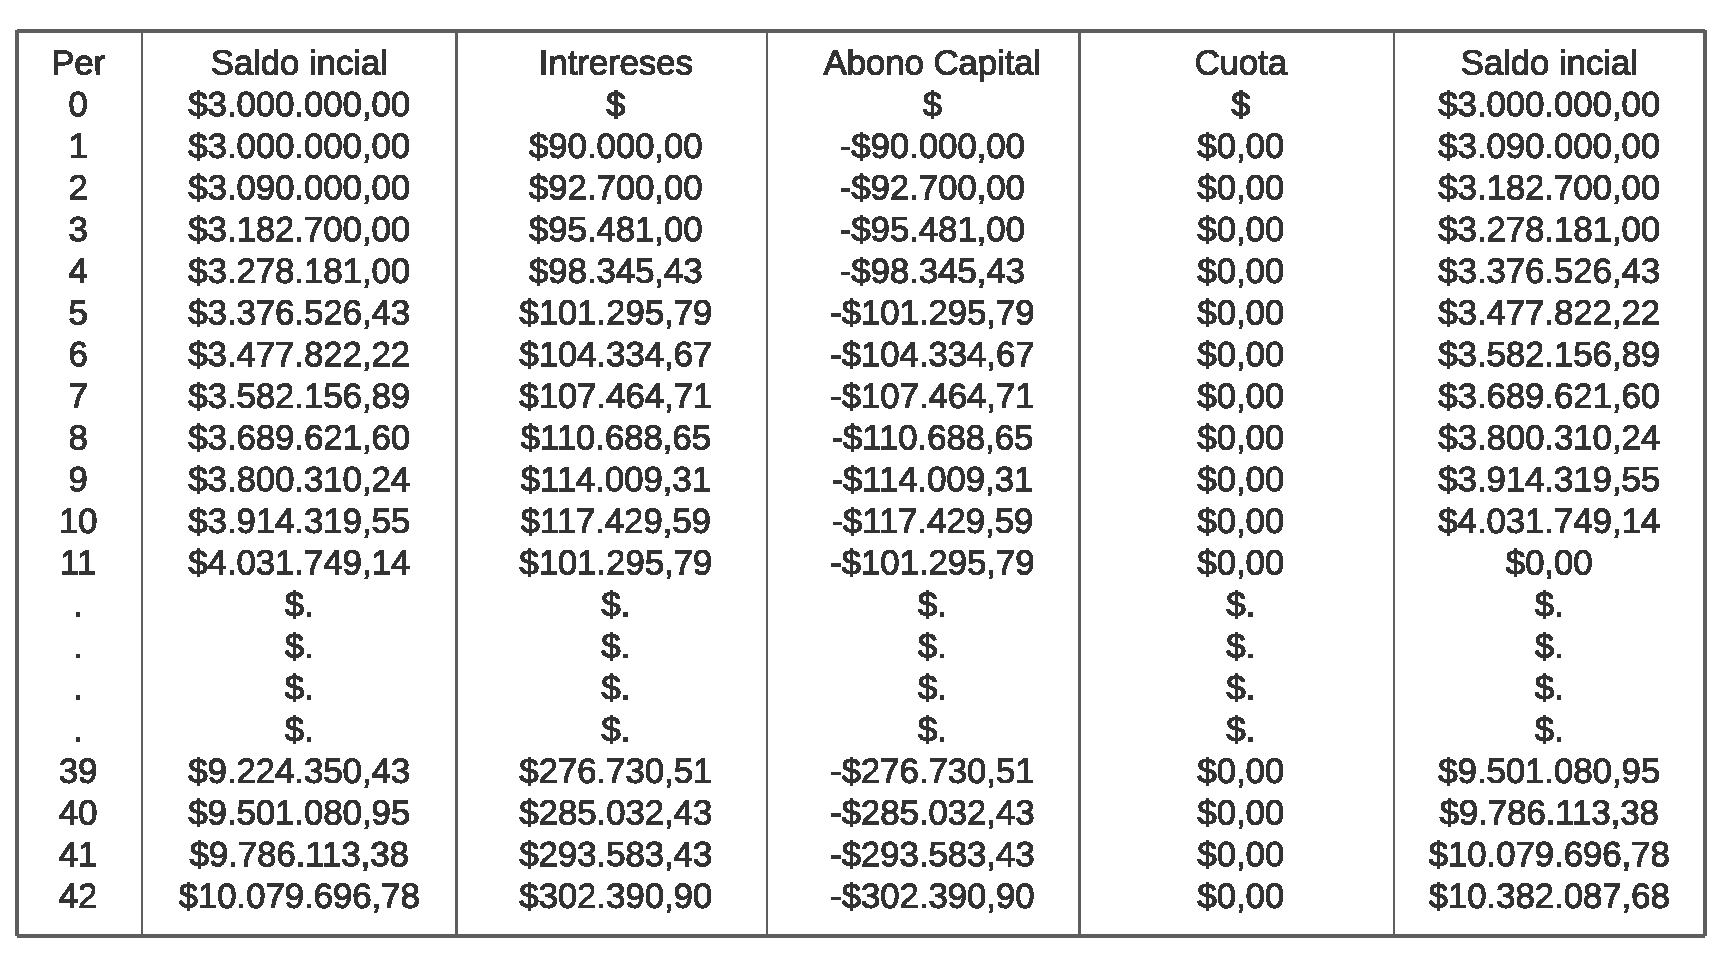
\includegraphics[trim=-5 -5 -5 -5 ,width=0.6\columnwidth]{12/tabla.pdf}} \\ \hline
  \multicolumn{2}{|c|}{\cellcolor[HTML]{FFB183}\textbf{3. Aplicación de funciones}}                                                                                                                     \\ \hline
  \multicolumn{2}{|p{\columnwidth}|}{Se aplicará la función Buscar objetivo de la siguiente forma:}                                                                                                     \\
  \multicolumn{2}{|c|}{ 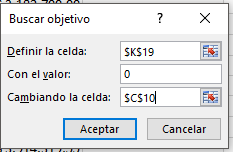
\includegraphics[trim=-5 -5 -5 -5 ,width=0.4\columnwidth]{12/excel1.png}}                                                                                                       \\ \hline
  \multicolumn{2}{|c|}{\cellcolor[HTML]{FFB183}\textbf{4. Gráfico}}                                                                                                                                     \\ \hline
  \multicolumn{2}{|c|}{ 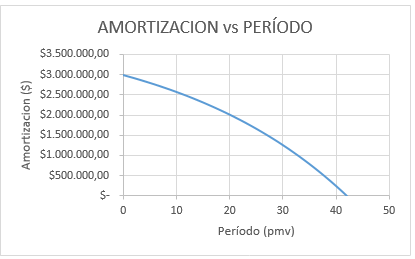
\includegraphics[trim=-5 -5 -5 -5 ,width=0.65\columnwidth]{12/grafico.png}}                                                                                                     \\ \hline
  \multicolumn{2}{|c|}{\cellcolor[HTML]{FFB183}\textbf{5. Respuesta}}                                                                                                                                   \\ \hline
  \multicolumn{2}{|c|}{De esta forma se obtiene el valor de  COP 126.575,02 para la cuota.}                                                                                                                \\ \hline
 \end{longtable}
 %\newline \newline %USARLO SI CREES QUE ES NECESARIO
\end{center}

%Tabla del ejercicio en latex por si alguna vez se necesita
%\begin{tabular}{|p{1cm}|p{2,5cm}|p{2,5cm}|p{2,5cm}|p{2,5cm}|p{2,5cm}|}
%\hline
%\textbf{Per} & \textbf{Saldo Inicial} & \textbf{Intereses} & \textbf{Abono Capital} & \textbf{Cuota} & \textbf{Saldo Final} \\ \hline



%0            &  COP 3.000.000,00         &  COP                  &  COP                      &  COP              &  COP 3.000.000,00       \\ \hline
%1            &  COP 3.000.000,00         &  COP 90.000,00        & - COP  90.000,00          &  COP 0,00         &  COP  3.090.000,00      \\ \hline
%2            &  COP  3.090.000,00        &  COP 92.700,00        & - COP 92.700,00           &  COP 0,00         &  COP 3.182.700,00       \\ \hline
%3            &  COP 3.182.700,00         &  COP 95.481,00        & - COP 95.481,00           &  COP  0,00        &  COP  3.278.181,00      \\ \hline
%4            &  COP 3.278.181,00         &  COP 98.345,43        & - COP 98.345,43           &  COP 0,00         &  COP 3.376.526,43       \\ \hline
%5            &  COP 3.376.526,43         &  COP 101.295,79       & - COP 101.295,79          &  COP 0,00         &  COP 3.477.822,22       \\ \hline
%6            &  COP 3.477.822,22         &  COP 104.334,67       & - COP 104.334,67          &  COP 0,00         &  COP  3.582.156,89      \\ \hline
%7            &  COP  3.582.156,89        &  COP 107.464,71       & - COP  107.464,71         &  COP 0,00         &  COP  3.689.621,60      \\ \hline
%8            &  COP  3.689.621,60        &  COP 110.688,65       & - COP 110.688,65          &  COP 0,00         &  COP  3.800.310,24      \\ \hline
%9            &  COP  3.800.310,24        &  COP 114.009,31       & - COP 114.009,31          &  COP  0,00        &  COP  3.914.319,55      \\ \hline
%10           &  COP 3.914.319,55         &  COP 117.429,59       & - COP 117.429,59          &  COP 0,00         &  COP 4.031.749,14       \\ \hline
%11           &  COP 4.031.749,14         &  COP 101.295,79       & - COP 101.295,79          &  COP 0,00         &  COP 0,00               \\ \hline
%.            &  COP  .                   &  COP  .               &  COP  .                   &  COP .            &  COP .                  \\ \hline
%.            &  COP  .                   &  COP  .               &  COP  .                   &  COP .            &  COP .                  \\ \hline
%.            &  COP  .                   &  COP  .               &  COP  .                   &  COP .            &  COP .                  \\ \hline
%.            &  COP  .                   &  COP  .               &  COP  .                   &  COP .            &  COP .                  \\ \hline
%39           &  COP 9.224.350,43         &  COP 276.730,51       & - COP 276.730,51          &  COP 0,00         &  COP 9.501.080,95       \\ \hline
%40           &  COP 9.501.080,95         &  COP 285.032,43       & - COP 285.032,43          &  COP 0,00         &  COP 9.786.113,38       \\ \hline
%41           &  COP 9.786.113,38         &  COP 293.583,40       & - COP 293.583,40          &  COP 0,00         &  COP 10.079.696,78      \\ \hline
%42           &  COP 10.079.696,78        &  COP 302.390,90       & - COP 302.390,90          &  COP 0,00         &  COP 10.382.087,68      \\ \hline
%\end{tabular}
%\end{center}
